% ****** Start of file apssamp.tex ******
%
%   This file is part of the APS files in the REVTeX 4.2 distribution.
%   Version 4.2a of REVTeX, December 2014
%
%   Copyright (c) 2014 The American Physical Society.
%
%   See the REVTeX 4 README file for restrictions and more information.
%
% TeX'ing this file requires that you have AMS-LaTeX 2.0 installed
% as well as the rest of the prerequisites for REVTeX 4.2
%
% See the REVTeX 4 README file
% It also requires running BibTeX. The commands are as follows:
%
%  1)  latex apssamp.tex
%  2)  bibtex apssamp
%  3)  latex apssamp.tex
%  4)  latex apssamp.tex
%
\documentclass[
%reprint,
%superscriptaddress,
%groupedaddress,
%unsortedaddress,
%runinaddress,
%frontmatterverbose, 
%preprint,
%preprintnumbers,
%nofootinbib,
%nobibnotes,
%bibnotes,
 amsmath,amssymb,
 aps,
%pra,
%prb,
%rmp,
%prstab,
%prstper,
%floatfix,
%twocolumn
]{revtex4-2}

% Packages
\usepackage{dcolumn}% Align table columns on decimal point
\usepackage{bm}% bold math
\usepackage[version=4]{mhchem}
\usepackage{stfloats}
\usepackage{color}
\usepackage{amssymb}
\usepackage{stmaryrd}
\usepackage{xcolor}
\usepackage{comment}
\usepackage{placeins}
\usepackage{graphics}
\usepackage{amssymb}
\usepackage{amsmath}
\usepackage{epsfig}
\usepackage{graphicx}
\graphicspath{{./figures/}}
\usepackage{epstopdf}
\usepackage{float}
\usepackage{tikz}
\usepackage{pbox}
\usepackage{array}
\usepackage{caption}
\usepackage{comment}
\usepackage{fancyhdr}
\usepackage{soul}
\usepackage{booktabs}
\usepackage{siunitx}
\usepackage[normalem]{ulem}
\usepackage{nomencl}
\makenomenclature

% \usepackage[numbers,sort&compress]{natbib}
% \bibliographystyle{abbrvnat}

\usepackage{subcaption}
\usepackage{hyperref}
\hypersetup{
    colorlinks=true,
    allcolors=blue,
    pdftitle={manuscript},
    % linkcolor=blue,
    % filecolor=magenta,      
    % urlcolor=cyan,
    % pdfpagemode=FullScreen,
    }
\usepackage{todonotes}
\setuptodonotes{inline}
% Set up cleveref (simpler references)
\usepackage{cleveref}
\crefname{equation}{Eq.}{Eqs.}
\Crefname{equation}{Equation}{Equations}
\crefname{table}{Tab.}{Tabs.}
\Crefname{table}{Table}{Tables}
\crefname{figure}{Fig.}{Figs.}
\Crefname{figure}{Figure}{Figures}
\crefname{section}{Sec.}{Secs.}
\Crefname{section}{Section}{Sections.}
\newcommand{\crefrangeconjunction}{--}

% Author defined commands and environments
\newcommand{\FS}{\textit{FlameSheet}$^\text{TM}$\ }
\renewcommand*{\vec}[1]{\ensuremath\mathbf{#1}}
\newcommand{\pd}[2]{\ensuremath\frac{\partial #1}{\partial #2}}
\newcommand{\dd}{\ensuremath\mathrm{d}}
\newcommand{\me}{\ensuremath\mathrm{e}}

\begin{document}

\title{Documentation of \textit{syntheticTurbulenceInlet}\\ -- the new inlet boundary condition for OpenFoam-12 that generates synthetic turbulence}
\author{Hursanay Fyhn and Eirik Fyhn}
\affiliation{SINTEF Energy Research}
\email{hursanay.fyhn@sintef.no}

\date{\today}

% \begin{abstract}
% \end{abstract}

%\keywords{Suggested keywords}%Use showkeys class option if keyword
                              %display desired
\maketitle

 \tableofcontents

%%==============================================================================
\section{Guide}%
\label{sec:guide}
\subsection{Setup}%
\label{sub:Setup}

Here are the steps on getting the BC up and running on your local OpenFoam-12.
Open a terminal and do the following:
\begin{enumerate}
  \item Clone the repository to any folder (given that you have access) by typing:\\ \textit{git clone git@gitlab.sintef.no:Hursanay.Fyhn/syntheticturbulenceinlet.git}
  \item Go into the cloned folder by typing\\ \textit{cd syntheticTurbulenceInlet}
  \item Source you local OpenFoam-12 the way you normally source it.
  \item Compile the boundary condition and add it to the list of boundary conditions for your OpenFoam-12 by typing:\\ \textit{wmake}
    \\ (ignore the message about .H files already existing)
  \item You can now use the BC like any other, just remember to source the relevant library by adding this line to your controlDict:\\
    \textit{libs (``libsyntheticTurbulenceInlet.so'');}
  \item Within the cloned directory, you will find a folder titled tutorials. Try out the tutorial cases for the four different geometry modes inside the tutorials folder.
\end{enumerate}

\subsection{Parameters}%
\label{sub:Parameters}

\begin{itemize}
  \item \textit{massFlowMode} (bool) (optional)\\
    Choose if you want to specify a massFlow (with true) or an Umean (with false).\\
    Default: false

  \item \textit{massFlow} (scalar, table, coded or other Function1 types) (required if massFlowMode is true)\\
    Total mass flow rate into the patch.

  \item \textit{Umean} (scalar, table, coded or other Function1 types) (required if massFlowMode is false)\\
    Mean speed into the patch.

  \item \textit{geometryMode} (annulus, disk, rectangle, channel or arbitrary) (required)\\
    Channel is rectangle with PBC in one direction. The purpose of the arbitrary mode is to generate turbulence on a patch with arbitrary shape, do not follow the DNS profiles unlike the other geometry modes due to constant $U$, $R$ and $L$.

  \item \textit{wallLongOrShort} (long or short) (optional)\\
    When \textit{geometryMode} is \textit{channel}, choose if the wall is on the long or the short side.\\
    Default: long

  \item \textit{arbitraryModeRadius} (scalar) (optional)\\
    When \textit{geometryMode} is \textit{arbitrary}, the use can choose the radius within which to generate turbulence.\\
    Default: The largest distance from the patch center.

  \item \textit{arbitraryModeCenter} (vector) (optional)\\
    When \textit{geometryMode} is \textit{arbitrary}, the user can choose the center coordinate.\\
    Default: geometrically averaged center coordinate of the patch.

  \item \textit{Utau} (scalar) (optional)\\
    Friction velocity\\
    Default: Utau is calculated from the expression for a smooth pipe. There is an absolute lower limit that maps the entire DNS profile over the entire width, and it can be forced by e.g. choosing a negative value.

  \item \textit{swirlNr} (scalar) (optional)\\
    Swirl number\\
    Default: 0

  \item \textit{d} (scalar) (optional)\\
    Eddy density (ratio of the sum of eddy volumes to the eddy box volume)\\
    Default: 1

  \item \textit{scale} (scalar) (optional)\\
    A scaling factor for $U'$\\
    Default: 1

  \item \textit{nCellPerEddy} (int) (optional)\\
    Minimum eddy length in units of number of cells\\
    Default: 1

  \item \textit{Lref} (scalar) (optional)\\
    Normalisation factor for integral-length scale\\
    Default: 1
    
  \item \textit{seed} (unsigned int) (optional)\\
    Seed for the random numbers\\
    Default: an arbitrary number

\end{itemize}

\subsection{Example usage}%
\label{sub:Example usage}

\noindent inlet\\
  \{\\
    type            syntheticTurbulenceInlet;\\
    geometryMode    annulus;\\
    massFlowMode    true;\\
    massFlow        2.53e-4;\\
  \}\\



%%===============================================================================
\section{Information}%
\label{sec:Information}
We have implemented a synthetic turbulence boundary condition for OpenFoam-12 inpired by the turbulent boundary condition called turbulentDFSEMInlet (referred to as DFSEM from here on) that exists in the ESI version and not in the foundation version of the OpenFoam.

There are some things in our implementation that are the same as in the paper by Poletto et. al. (referred to as the paper from here on), but different from DFSEM where there might have been errors in the implementation.
First, we fixed the error where the normalization step was done before the application of the rotation matrix for Reynolds stress tensor $R$, so that it matches the paper.
We fixed this error which made the eddies elongated in the right direction, the flow direction.
Second, we changed the expression for $U'$ which is the fluctuation in the velocity $U$.
The functional form of the expression for $U'$, in other words, the dependence of $U'$ on the radius of the eddy, is the same as in the paper. 
In DFSEM, this was different than the expression in the paper.

In addition, in our implementation, there are things that are different and improved from both the DFSEM and the paper. 
Recalculating the expressions in the paper gave us different scaling factors in the expression for $U'$.
The new expression gave largely improved results.

Determined to make our BC more user friendly, we have implemented several features that did not exist in DFSEM.
Firstly, we have implemented four of the most common geometries for the inlet that the user can choose between: an annulus, a disk, a rectangle and a channel.
We have implemented automatic detection of the dimensions and the directions of the geometry of the inlet patch for these four modes.
This mean the user does not need to specify the radii of the annulus and the disk, or the sides and the vertices of the rectangle and the channel.
For the channel mode, the user has the freedom to choose if the longest or the shortest edge is the wall, the other edges will then be assumed to be periodic, also in terms of the eddies. 

To use DFSEM, one needs to do some mapping and processing of the data beforehand. 
This is not necessary in our BC as we map the relevant information directly to the cells in OpenFoam.
Our BC also works regardless of the flow direction because we use the normal vector of the patch to determine the direction and we compute the Reynolds stress tensor etc. correctly inside the boundary condition rather than from external files.

There is a need to generate random numbers for the position of the eddies and the direction of the rotation of the eddies.
Random numbers in the code are are generated with Mersenne Twister using the same seed over all the processors to make sure that the same random number is generated.

In the DNS data files, the quantities are given as a function of the position $y$ or $y^+$. 
$y^+$ is the dimensionless position that is scaled with friction velocity $u_\tau$ and the kinematic viscosity $\nu$ as $y^+ = u_\tau y /\nu$.
We use $y^+$ instead of $y$ in mapping of the DNS data onto the geometry, as it gives us more flexibility due to it being scaled with the boundary layer thickness.
We do that by having friction velocity $u_\tau$ as a parameter.
In the code, $u_\tau$ is set to have an absolute lower minimum limit, that will map the entire profile of the DNS data over the entire width.
Larger $u_\tau$ makes the boundary layer thinner and the middle is filled in with a constant that is the half-width value from the data.
$u_\tau$ can also be spesified by the user, if not, it will be calculated by default by using the expression for a smooth pipe.

We have implemented the possibility to have a swirling velocity profile in the code. 
Swirl number $S$ is defined as
\begin{equation}
\label{eq:S1}
  S = \frac{\int_{A} \rho \bar u_x \bar u_\theta r \dd A}{\bar r \int_{A} \rho \bar u^2_x \dd A}
\end{equation}
$\rho$ is the density, $ \bar u_x$ is the mean velocity profile in the axial direction, $\bar u_\theta$ is the mean velocity profile in the angular direction, $r$ is the radius, $A$ is the area, and $\bar r = (r_i+r_o)/ 2$ where $r_i$ is the inner radius, $r_o$ is the outer radius. 
To have a $\bar u_\theta$ that follows the shape of $\bar u_x$ and a velocity profile that does not have a curl that diverges when $r_i = 0$, we choose a form 
\begin{equation}
\label{eq:utheta}
  \bar u_\theta = f_\theta r \bar u_x 
\end{equation}
where $f_\theta$ is a constant.
Inserting \cref{eq:utheta} into \cref{eq:S1} gives
\begin{equation}
  \label{eq:S2}
  S = \frac{ f_\theta\int_{A} \rho \bar u_x^2 r^2 \dd A}{\bar r \int_{A} \rho \bar u^2_x \dd A}
\end{equation}
In the code, for a user given $S$, $f_\theta$ is calculated from \cref{eq:S2} and inserted into \cref{eq:utheta} to find $\bar u_\theta$. 

% \begin{equation}
%   S = \frac{\int_{r_i}^{r_o} \rho \bar u_x \bar u_\theta r^2 \dd r}{\bar r \int_{r_i}^{r_o} \rho \bar u^2_x r \dd r}
% \end{equation}

We have also added the functionality to specify mass flow rate instead of a mean speed.

To summarize, the results produce a better match to the original DNS data than DFSEM due to the recalculated expression.
Also, there are many additional features that have been added to our implementation that improves the ease of use. 

%%===============================================================================
% Short about how U' = U - Umean is calculated: {{{ %
% - Eddies are elongated spheroids with radii: vec sigma = [sigmay, sigmaz(=sigmay), sigmax]
% - the longest direction sigmax is calculated from L and the other two directions are scaled with a gamma that is sqrt(an integer between 1 and 8) so they are smaller than sigmax.
% - the principal coordinate system of an eddy, i.e. the directions in which the sigmas are defined, is along the eigenvectors of R.
% - the longest length (sigmax) is along the eigenvector of R with the largest eigenvalue. By sorting in the code that eigenvector is always pointing in the direction nr 3 locally (z-direction locally). 
% The eigenvector of R with the largest eigenvalue seems to be in the flow direction (u in Ruu) in the data file. Since the code places that direction at the end in the local coordinate system, our coordinate system has to be rotated so that the flow direction is z before scaling.  
% - we did not know that the longest direction is the flow direction beforehand, we just knew that the three lengths in vec sigma is defined along the eigenvecs of R and we rotated to that coordinate system and scaled and calculated U'. It seems from the results that the longest direction happends to be in the flow direciton. 

% - They are placed at (semi) random position within +- maxSigmax from the patch, calculated from L.

% - nr of eddies is determined by this: total eddy volume = v0 = 2*maxSigmax* inlet-area

% - At a point of the inlet, to find the contribution from one eddy to the U' at that point:
%   We first transform to the eddie's principal coordinate system, defined by the eigenvectors of R at that point. Which means R is diagonal there and the covariances are zero, which makes the expression for U' easy in this coordinate system. Also, the expression for U' from the paper is defined in the coordinate system that is scaled with the size of the eddy so where the eddy is a sphere with radius one because it is easiest like that. In that coordinate system, if the point of interest lies outside the radius 1 than U' contribution is zero from that one eddy.

% - The eddies move forward with time, so their contribution to the patch changes with time. When they pass maxSigmax, they are switched out with a different eddy (semi) randomly placed within +- maxSigmax from the patch (DFSEM had only +maxSigmax which made less sense).
% }}}  %

%%===============================================================================
\section{Test results }%
\label{sec:Results}

\Cref{fig:URL_x} shows the time averaged quantities measured over a line at various positions $x$. 

\begin{figure}[ht]
  \centering
  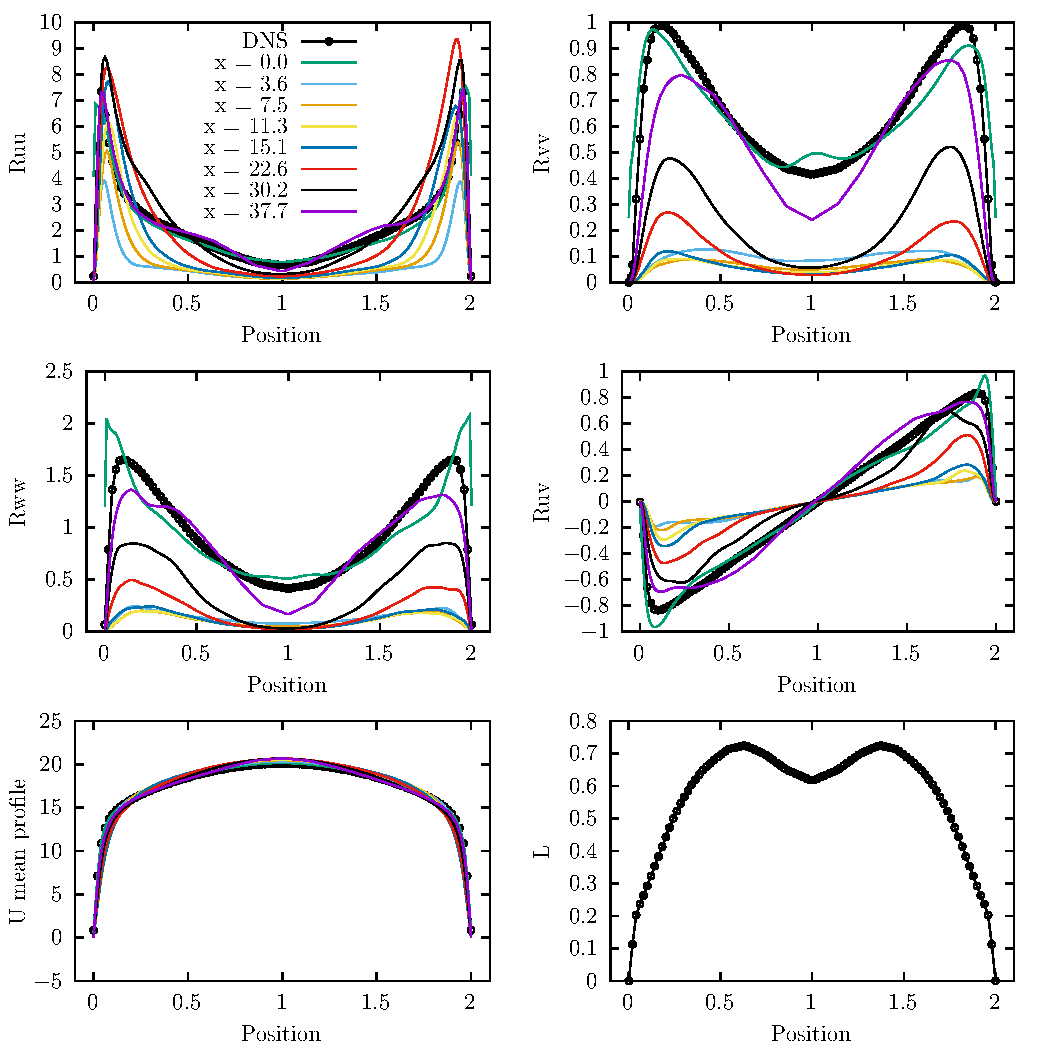
\includegraphics[width=1.0\textwidth]{URL_x.pdf}
  \caption{The time averaged quantities measured over a line at various positions $x$. }
  \label{fig:URL_x}
\end{figure}


%%===============================================================================
\end{document}
